\documentclass[a4paper, 10pt]{article}
\usepackage[UTF8]{ctex}
\usepackage{subfigure}
\usepackage[graphicx]{realboxes}
\begin{document}
  \title{国际金融笔记}
  \author{亦可}
  \maketitle
\section{汇率}
\subsection{有效汇率}
$$E_{eff}=\sum E_i\frac{Trade_i}{Trade}$$
$$\frac{\Delta E_{eff}}{E_{eff}}=\sum \frac{\Delta E_iTrade_i}{E_iTrade}$$

\subsection{固定汇率制度}
\noindent 美元化:小国维持独立货币成本过高;货币改革结果糟糕导致本国货币信用大跌等

\noindent 货币局制度:需要足够多的美元储备;无限制兑换;固定汇率制度

\noindent 爬行汇率制


\subsection{浮动汇率制度}

\subsection{外汇市场的参与者}
\noindent 三种私人参与者:商业银行、跨国公司、公募基金

\noindent 政府行为:资本限制、建立固定汇率贸易市场(可能会出现黑市、外汇干预

\subsection{即期交易}
\subsection{衍生品}
\noindent 远期(主要)、调期、期货、期权
\subsection{套利}
\noindent 无风险套利CIP:
$$1+i_d=\frac{F_{d/f}}{E_{d/f}}(1+i_f)$$
风险套利UIP:
$$1+i_d=\frac{E^e_{d/f}}{E_{d/f}}(1+i_f)$$
费舍效应:
$$i_{nominal}=i_{real}+\pi ^e$$
$$i_d=i_f+\frac{\Delta E^e_{d/f}}{E_{d/f}}$$

\section{汇率的货币理论}
\subsection{购买力平价}
绝对购买力平价:
$$E_{d/f}=\frac{P_d}{P_f}$$
相对购买力/真实汇率:
$$q_{d/f}=\frac{E_{d/f}P_f}{P_d}$$
真实汇率大于1,说明本币被高估,外币被低估。


\noindent 相对购买力平价:
$$\frac{\Delta E^e_{d/f}}{E_{d/f}}=\pi_d-\pi_f$$
对绝对购买力平价的偏离:交易成本、非交易品、不完全竞争和法律限制、价格粘性等
\subsection{货币数量论}
$$M_{demand}/P=LY$$
其中M为名义货币需求,M(demand)/P或LY为实际货币需求,Y为真实收入,PY为名义收入。货币供给为给定外生变量。货币数量论是为了给出价格的决定。
$$P=\frac{M}{LY}$$
故有汇率的表示:
$$E_{d/f}=\frac{M_d/M_f}{L_dY_d/L_fY_f}$$
$$\frac{\Delta E^e_{d/f}}{E_{d/f}}=\mu_d-\mu_f-(g_d-g_f)$$
其中$\mu$为名义货币供给的增长率,g为真实产出的增长率

\subsection{理论的补充-一般模型}
\noindent L不一定为常量,一般的有$L=L(i)$为减函数

\noindent 真实利率不变。利率决定于通胀预期。
$$E_{d/f}=\frac{M_d/M_f}{L(i)_dY_d/L(i)_fY_f}$$
一般来说,外生的突变都发生在货币供给的变化上。一般来说,Y是不变的。这是解题关键。L与i无关时,M的变化直接推得P的变化推得汇率的变化。L与i有关时,M的0阶变化直接导致P的0阶变化,与前述相同。M的增长率的变化导致通胀率的变化。通胀率的变化导致i的变化导致L的变化,导致P发生0阶突变。
\section{汇率的资产理论}
\subsection{理论}
\noindent 由UIP,未来预期汇率和国内外利率决定了即期汇率,UIP可以用来确定收益-汇率图上的DR与FR曲线交点

\noindent 三种冲击:本国利率变化,外国利率变化,未来预期汇率的变化

\noindent 一般的货币数量论给出利率-真实货币需求(供给)图的两条线和交点。

\noindent 两种冲击:真实收入Y的冲击和实际货币供给M的冲击

\noindent 假设:价格粘性、名义利率可调

\subsection{短期和长期}
\noindent 短期的冲击不会改变预期,长期的冲击会改变预期。短期价格粘滞,长期价格灵活。长期的冲击在短期会出现超调。短期,价格粘滞,外生变量的改变会唯一地确定利率。长期,价格灵活可变,利率会回到最初水平(利率的回归性)于是长期的价格就被确定。

\section{汇率政策和三元悖论}
\subsection{名义锚}
\noindent 名义锚是为了锁定通胀率。

\noindent 汇率锚定

\noindent 相对PPP给出$\pi_d=\frac{\Delta E}{E}+\pi_f$,与一个通胀稳定的国家之间保证恒定的贬值率即可保证通胀稳定。

\noindent 货币供给锚定

\noindent 根据货币数量论$\pi=\mu-g$,保证稳定的实际货币供给增长率即可保证稳定的通胀率。缺点是g可能变化,g变化时该做法失效。实际产出水平高增长期,按照该策略进行锚定,实际通胀效果可能低于预期希冀通胀。

\noindent 利率锚定

\noindent 费舍效应给出$\pi=i-i_{real}$,控制利率即可控制通胀。


\subsection{悖论}
\noindent 固定汇率(外生未来预期汇率与即期汇率的关系)、国际资本的流动性(外生UIP)、货币政策的独立性(外生利率的自主决定)三者不可兼得。

\section{国际收支:账户}
\noindent 支出法、生产法、收入法
$$GNE=C+I+G$$
$$GNE+TB=GDP$$
$$GDP+NFIA=GNI$$
$$GNI+NUT=GNDI=Y$$
$$CA=TB+NFIA+NUT$$
$$BOP:CA+KFA+ERR=0$$
$$S=Y-C-G=I+CA$$
$$FA=EX^H_A-IM^H_A+EX^F_A-IM^F_A$$
$$S=Y-T-C+T-G=S_1+S_2$$
资本账户描述资本转移,即所有权的转移,比如中国在意大利的债券被中国免除等,以及专利、版权等非金融资产的收买,金融账户描述金融资产交易(也包括土地等固定资产的交易)。

\noindent home和foreign asset表示位置在本国还是外国,金融账户等于对外负债的增加加外部资产的出口,等于对外净负债

\subsection{BOP的推导}
\noindent 国民收入用来支出,除了总支出以外还有金融资产的部分。故有
$$GDNI+KFA=GNE$$
得到BOP。
\subsection{复式记账原理}
\noindent 每一笔账都会分别记在某个地方的借方和另一个地方的贷方。


\noindent 一个中国人向美国出售的一美元的苹果。这时,经常账户中商品与服务一栏的贷方记入+1,金融账户的对外资产一栏的借方计入-1


\noindent 一个中国人向美国捐赠一美元。这时,经常账户中转移一栏的借方记入-1,金融账户中对外资产的贷方+1


\noindent 一个中国人向美国捐赠价值一美元的货物。此时应分为两步看。第一步是捐赠一美元,第二步是美国向中国购买价值一美元的商品。此时,金融账户发生一次消长,最终呈现为经常账户的借方和贷方各有1美元

\noindent 一个中国人购买价值一美元的美股。此时,中国的对外资产形式发生一个转换,因此两笔账分别在金融账户的借方和贷方

\noindent 中国免除一美元的美国债务。此时,资本账户的借方记入-1,金融账户的贷方计入1

\subsection{外部资产}
\noindent 资本交易带来的外部资产变化$-FA$

\noindent 估值效应带来的外部资产变化,即资本利得,由汇率或利率变化导致

\noindent 恒等式:
$$\Delta W=-FA+VE=CA+KA+VE$$

\section{金融开放的好处:消费平滑}

\subsection{长期预算约束}

\noindent 模型假设:价格完全可调,只存在一种真实商品和一种真实资产。忽略经济的货币面的影响(汇率),分析全部基于真实变量。

\noindent 本国是小型开放经济体,只能被动接受价格,不能影响价格。

\noindent 真实利率为r

\noindent 无资本转移和捐赠行为,无资本账户

\noindent 经常账户中只有要素收入和净出口

\noindent 一个国家初始有一笔对外资产$W_0$,此时有
$$\Delta W_t=TB_t+NFIA=TB_t+rW^*_{t-1}$$
$$W_{t}=TB_t+(1+r^*)W_{t-1}$$
$$W_{t-1}=\frac{W_t}{1+r^*}-\frac{TB_t}{1+r^*}$$
长期预算约束要求,最终这个玩意得为0,你得还清贷款,即最远的W为0,有:
$$W_{0}=(1+r^*)W_{-1}+TB_0=-\frac{TB_1}{1+r^*}-\frac{TB_2}{(1+r^*)^2}+\dots$$
此即长期预算约束,即:
$$-(1+r^*)W_{-1}=\sum_{i=0}^n\frac{TB_i}{(1+r^*)^i}$$
debtor是对外资产为负的国家,需要有正的经常账户以满足长期预算约束,creditor是对外资产为正的国家,刚好相反。

\noindent 由于$TB=GDP-GNE$,有:
$$-(1+r^*)W_{-1}=\sum_{i=0}^n\frac{GDP_i-GNE_i}{(1+r^*)^i}$$
\subsection{美国的案例}
\noindent 其它国家持有的是美国的债券。美国持有的是其它国家的直接投资。美国八十年代开始成为一个债务国,外部资产为负,这说明美国的要素收入$\Delta W=r^*W$应该为负,但是实际上美国的外部财富变化在这一时期为正。是因为美国在计算外部资产变化时的利率和计算外部负债变化时的利率不同。此时美国的外部财富变化为:
$$\Delta W_N=TB_N+r^*W_{N-1}+(r^*-r^0)L+KG$$
学者统计,KG大概在1.5个百分点,利差所得大概在0.5个百分点,因此美国相对其它国家每年有2个百分点的净利润


\subsection{新兴市场的困境}
\begin{figure}[h]
  \centering 
  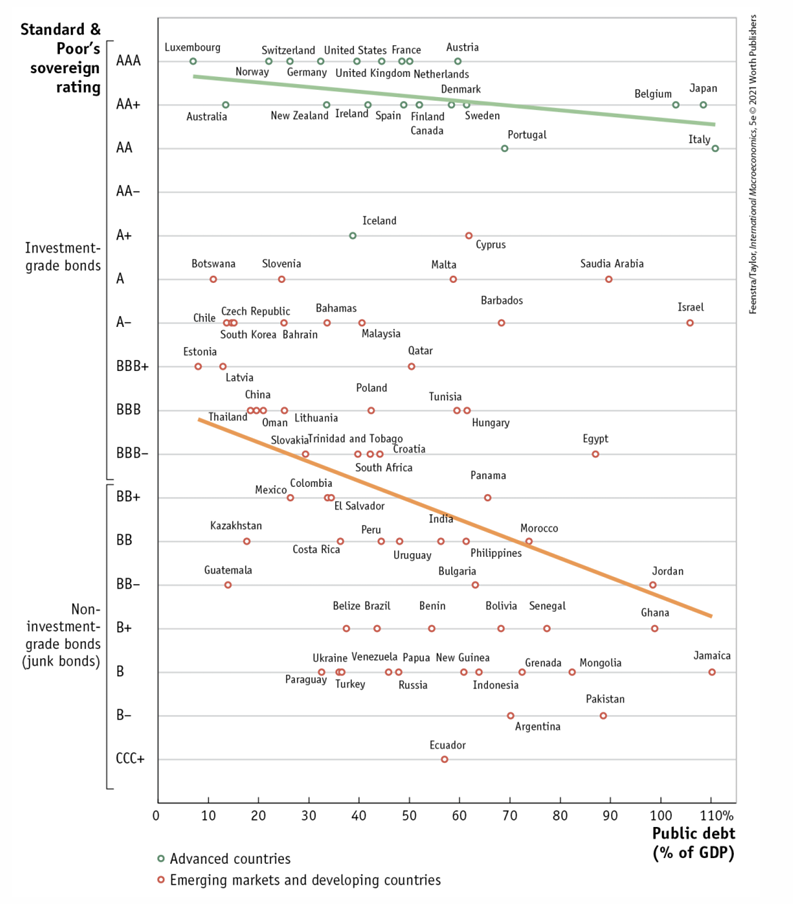
\includegraphics[height=10.0cm,width=12.0cm]{pic1.png}
  
  \caption{风险评级和债务率的线性拟合}
  \label{1}
  
  \end{figure}
  
\noindent 可以看到,新兴市场增加一单位债务引起的风险评级下降(主权信用下降)要大于发达市场。(高风险债券一般收益率也更高)

\subsection{资本骤停}
\noindent 指资本和金融账户瞬间出现萎缩。即外部流入的资金大幅减少。出现资本骤停的国家,一方面很难在国际市场进行融资,另一方面也很难用新的融资来还债。由此大幅影响一国经济。

\subsection{消费平滑}
\noindent 在面临冲击时,通过国际借贷可以让消费变得稳定。

\noindent 假设:只需要一种生产要素labor,不需要投资。每个单位为了最大化福利,会选择每期相同的消费。消费满足预算约束。消费从0期开始,没有初始负债。真实利率为外生给定变量$r^*$,此时预算约束变为:
$$0=\sum_{i=0}^n\frac{GDP_i-GNE_i}{(1+r^*)^i}$$
\noindent GDP是会面临冲击的。但总之是被“预知”的。你总可以首先算出GDP的现值,然后根据长期预算约束来安排消费。然后得到每年的TB和外部资产增加NFIA。

\noindent 一般化来说,我们认为初始外部资产为0的开放经济体,在第0年受到$\Delta Q$的生产减少冲击,此后恢复正常,那么每年消费应该减少:
$$\Delta C=\frac{r}{1+r}\Delta Q$$

\section{金融开放的好处:有效投资和风险规避}
\subsection{有效投资}
\noindent 加入投资项,长期预算约束变为:
$$-(1+r^*)W_{-1}=\sum_{i=0}^n\frac{GDP_i-GNE_i}{(1+r^*)^i}$$
初始财富为0,有:
$$0=\sum_{i=0}^n\frac{GDP_i-GNE_i}{(1+r^*)^i}$$
其中$GNE=C+I$,同样的,I和有了这笔投资之后每年的产出是外生给定的,根据长期预算约束和消费平滑可以计算出每年的消费值。

\noindent 一般化的理论为:
$$\frac{\Delta Q}{r}=\Delta C(1+1/r)+\Delta K$$
其中$\Delta K$为第零年的投资值,有效投资条件:
$$\frac{\Delta Q}{r}>\Delta K$$
此时投资能导致除了投资以外现值的增加(好好理解这句话),就是有效的,也只有在该条件下投资才会进行。有$MPK=\Delta Q/\Delta K$为边际投资收益。
\subsection{挪威的案例}
\noindent 1970年代,挪威大额投资于在海洋开采石油。挪威从开放经济中得到了好处,具体表现为它经受了一个大额的经常账户赤字以进行投资。在最夸张的时候,挪威的经常账户赤字达到了GDP的十分之一。
\subsection{卢卡斯悖论}
\noindent 发展中国家能有机会获得先进国家的技术。如果政策变化,允许资本的大额跨国流动,那么资本应该会蜂拥于发展中国家。这是因为发展中国家的边际产出比较高。

\noindent 假设生产函数为$Q=AK^\theta$,其中$\theta$表示资本对于生产的贡献,一般取为1/3,Q为人均产出,K为人均资本
$$MPK=q\theta/K$$
为什么资本现实中不流向发展中国家?

\noindent 是因为发展中国家和发达国家有不同的生产率A,在前面的讨论中,不同的国家的q和k都满足由同一对A和$\theta$组成的约束,也就是q和k中只有一个是需要给定的,但是实际情况是不同国家的A不同,q和K都需要外生给定才能计算出不同国家之间A的差距。

\noindent 真实利率r就是世界性的资本边际产出,做题的时候可以用来替换富国资本边际产出的位置。

\subsection{风险规避}
\noindent 多元化投资可以通过分摊风险以帮助在冲击来临时平滑冲击。通过多元化投资,国家可以减少收入的消失,而不需要任何借贷款。考虑两个国家A和B,它们有不对称的收入波动。两个可能的状态:
 $$state1=badA+goodB$$
 $$state2=goodA+badB$$
 每种状态有一个给定的发生概率。并且每个国家分别有一定比例的资本收入和劳动收入,如下图:

\begin{figure}[h]
  \centering 
  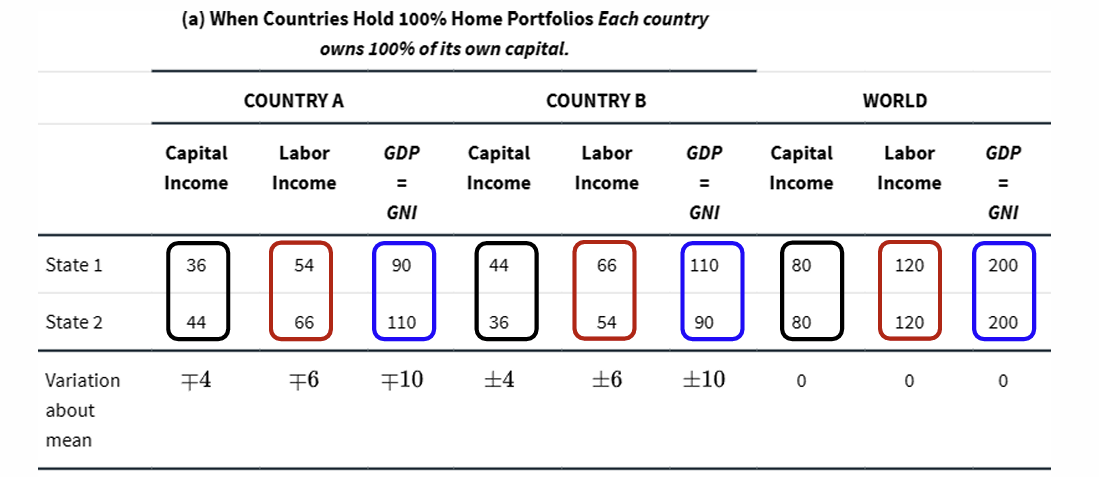
\includegraphics[height=6.0cm,width=12.0cm]{pic2.png}
  
  \caption{各国持有本国的百分百股权}
  \label{2}
  
  \end{figure}
或者,每个国家都持有本国和外国各一半的股票:

\begin{figure}[h]
  \centering 
  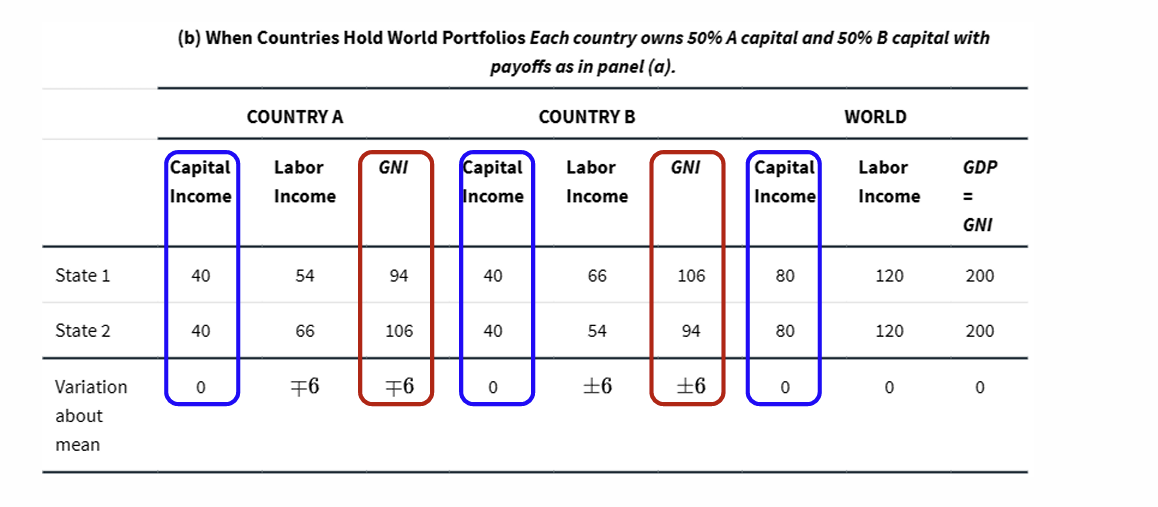
\includegraphics[height=6.0cm,width=12.0cm]{pic3.png}
  
  \caption{各国持有本国和外国各百分之五十股权}
  \label{3}
  
  \end{figure}
已经足够明了。还可以一般化讨论:两个国家是零和还是共享还是混杂?
\section{产出、汇率和宏观政策}
\noindent 外国经济用“ROW”表示。假设:短期价格不变;预期通胀为零;所有的量都同时是名义变量也是实际变量;政府花费G和收税T由政策给定;外部产出和外部利率给定;要素收入和转移为零,经常账户等于净出口。
$$D=C+I+G+NX$$
$$C=C_0+MPC(Y-T)$$
I(i)为向下倾斜曲线。定义真实汇率:
$$q=\frac{E_{d/f}P_f}{P_d}$$
q的变化,内外产出的变化都会影响净出口。且此时的有效汇率是真实汇率的加权平均。

\subsection{货品市场-IS曲线}
$$Y=G+I(i)+C(Y-T)+NE(q,Y-T,Y^*-T^*)$$
\begin{figure}[h]
  \centering 
  
\includegraphics[height=8.0cm,width=12.0cm]{pic4.png}
  
  \caption{货品市场}
  \label{4}
  
  \end{figure}

\noindent 当利率下降时,发生如图所示移动,至于为什么斜线斜率小于1,是因为首先边际消费小于1,其次一单位的收入增加要有一部分投入于负的净出口,因此斜率一定小于1大于零。

\noindent 由该图上的利率变化可以得到IS曲线。导致IS曲线移动的因素:







\end{document}